%!TEX root = ../AST208-notes.tex

\section{Electromagnetic radiation is quantized}

Electromagnetic radiation---light---is carried by massless particles known as \emph{photons}. Being massless, they travel at a speed $c$ in all frames.  The energy of a photon depends on its frequency $\nu$: $E_{\nu} = h\nu$. Since $\nu = \lambda/c$, we can also express the energy of a photon as $E_{\lambda} = hc/\lambda$. When matter absorbs or emits radiant energy, it does so by absorbing or emitting photons.

\begin{exercisebox}
On a very dark night, the eye can make out stars down to visual magnitude $V\approx 6$. Given that the sun has $V=-26.71$ and that the flux from the sun in $V$-band is approximately $\val{10^{3}}{\unitstyle{W}/\meter^{2}}$, estimate the radiant flux from this $V=6$ star.  If the $V$ band photons have an average $\lambda = \val{550}{\nano\meter}$, how many photons from this barely visible star enter your pupil and strike your retina each second?
\end{exercisebox}

Image we shine a monochromatic (just one wavelength) beam of light at a tinted piece of glass (your sunglasses, for example).  The light that emerges on the other side is the same color---meaning it has the same wavelength---but is dimmer. What are we to make of this? For the exiting light to be dimmer, some of the photons must have been absorbed. But which photons are absorbed? Since the photons are all identical, we must adopt a probabilistic viewpoint: each photon has a certain probability of being absorbed.

\section{The hydrogen atom}

The electrons bound to an atom or molecule also have a discrete set of energies. For example, the electron in a hydrogen atom only has energies
\begin{equation}\label{e.H-levels}
	E_{n} = -\val{13.6}{\eV}\times \frac{1}{n^{2}},
\end{equation}
where $n > 0$ is an integer known as the principal quantum number.  The energy of the lowest state, $n=1$, is negative: it takes \val{13.6}{\eV} to remove the electron from the atom.

Because the electrons in an atom can only have certain energies, the atom can only absorb or emit light at specific wavelengths, such that the energy of the photon matches the difference in energy between two levels.  For example, a hydrogen atom can absorb a photon of energy
\[
	E_{1\to2} = -\val{13.6}{\eV} \left(\frac{1}{2^{2}} - \frac{1}{1^{2}}\right)
		 = \val{10.2}{\eV}
\]
corresponding to the energy required to move the electron from  $n=1$ to $n=2$.

The wavelengths that can be emitted or absorbed by a hydrogen atom at rest can be found by substituting $E = hc/\lambda$ into equation~(\ref{e.H-levels}):
\begin{equation}
	\lambda_{m\to n} = \lambda_{0}\left(\frac{1}{n^{2}}-\frac{1}{m^{2}}\right)^{-1},
\end{equation}
where $\lambda_{0} = \val{91.2}{\nano\meter}$.
The transitions to the lowest levels are named after their discoverers: Lyman for $m\to1$, Balmer for $m\to2$, Paschen for $m\to3$. A greek letter is used to denote the higher state: for example Lyman $\alpha$ (abbr.\ Ly$\alpha$) means $2\to1$, with $\lambda_{\mathrm{Ly}\alpha} = \val{121.6}{\nano\meter}$.  The first line transition in the Balmer series is $3\to2$, and is designated H$\alpha$: $\lambda_{\mathrm{H}\alpha} = \val{656.3}{\nano\meter}$. The levels of the hydrogen atom are shown in Fig.~\ref{f.H-spectrum}. The first 50 lines for the Lyman ($m\to1$), Balmer ($m\to2$), and Paschen ($m\to3$; note the $4\to2$ transition is outside the plot range) are shown.

\begin{figure}[htbp]
\includegraphics[width=\linewidth]{H-spectrum}
\caption{Spectral lines of neutral hydrogen. 
\label{f.H-spectrum}}
\end{figure}

\section{Diffraction Gratings}

To look at the different wavelengths in the light from a source, we use a diffraction grating, which is a series of fine, closely spaced lines etched on a surface.  When light is projected onto the grating, it is reflected from the lines in all directions.  Along a given direction, the light from two adjacent lines will travel a slightly different distance: if the spacing between lines is $d$, the extra distance is $d\sin\theta$, where $\theta$ is the angle between the incident and reflected rays. Because of this different path length, when the light reaches a distant detector it is a jumble of waves of different phases. When the waves are added together, the peaks and troughs cancel, and the result is that the wave is reduced in amplitude.  If, however, the extra path length is a multiple of the wavelength then the peaks align producing a bright spot. That is, at angles satisfying
\begin{equation}
d\sin\theta = m\lambda,
\end{equation}
bright spots are produced.This situation is depicted in Fig.~\ref{f.diffraction-grating} for $m=1$.

\begin{marginfigure}
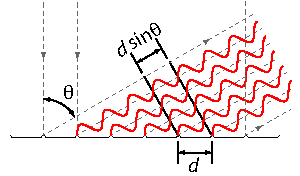
\includegraphics[width=\linewidth]{diffraction-grating}
\caption{A diffraction grating.
\label{f.diffraction-grating}}
\end{marginfigure}

Different wavelengths produce their bright spots at different angles.  If, for example, the angle $30^{\circ}$ corresponds to a bright spot for $\lambda=\val{650}{\nano\meter}$, then the angle for $\lambda=\val{400}{\nano\meter}$ is
\[
\theta_{400} = \arcsin\left(\sin 30^{\circ}\times\frac{\val{400}{\nano\meter}}{\val{650}{\nano\meter}}\right) = 18^{\circ}.
\]
The closer the lines are spaced, the more the light is dispersed. Typical gratings range from a few hundred to a few thousand lines per millimeter. A good home example of a grating is a CD: the tracks act as the lines on a grating.

\begin{exercisebox}
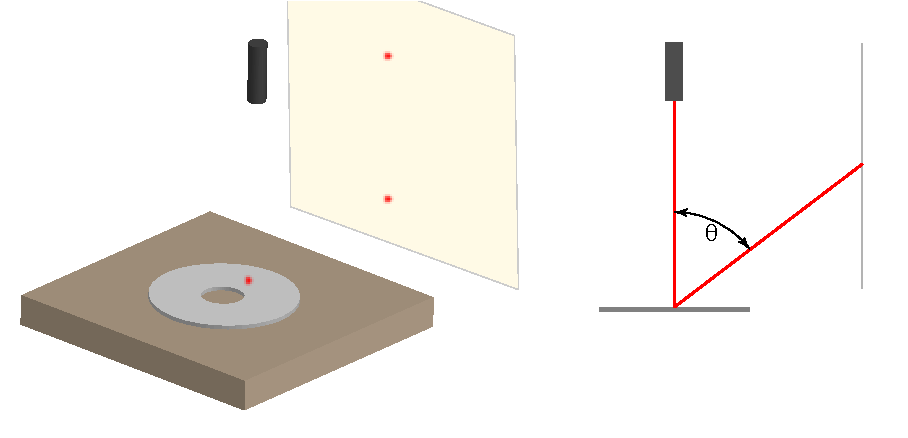
\includegraphics[width=\linewidth]{cd-diffraction-AST208}
You shine a red laser pointer ($\lambda=\val{650}{\nano\meter}$) onto a face-up CD, and observe that two dots appear on a blank screen, as shown above. The laser beam is vertical and the two dots that appear on the screen are at angles $23^{\circ}$ and $52^{\circ}$ from the vertical. There is no third dot appearing above these two. From the information given, calculate the spacing between the tracks on the CD.
\end{exercisebox}

For a telescope, there is an additional complication: we don't have a single source, but rather an image of the entire field of view. To restrict our field of view, we overly our grating with a slit, as shown in Figure~\ref{f.slit-and-grating}. The width of the slit is matched to the seeing so that if projects a line of light onto the diffraction grating. The dispersed light thus makes a two dimensional image, with position along the slit along one axis, and wavelength along the other axis.

\begin{figure}[htbp]
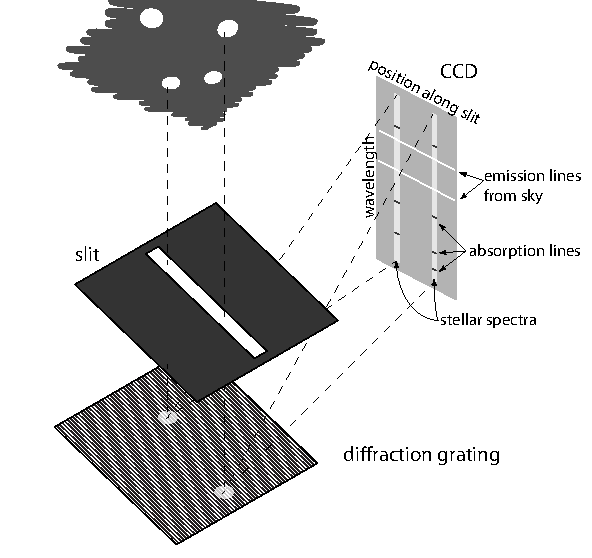
\includegraphics[width=\linewidth]{slit-and-grating}
\caption{Taking a spectrum of an astronomical object.
\label{f.slit-and-grating}}
\end{figure}

\section{Absorption and emission lines}
Now that we are taking spectra, what do we see?  Suppose we look at a tenuous cloud of hot gas, and there is no light source behind this cloud. Because the gas is hot, collisions between atoms will excite electrons into excited states. When these electrons make a transition to the ground state, a photon is emitted. Thus, when we take a spectrum of the light from this cloud, we expect to see a series of discrete, bright lines at those frequencies. This is an \emph{emission line spectrum}. 

Emission lines are also produced in Earth's atmosphere from a variety of sources: for example collisions of molecues with cosmic rays and recombination of ions and electrons that had been photoionized by sunlight.

Conversely, suppose we have gas that is backlit by a strong source of photons---think of the atmosphere of a star. As the photons go through the gas, some are absorbed. Thus, the spectrum is a continuous blend of light, with darker lines corresponding to the absorption in the atmosphere.  This is an \emph{absorption line} spectrum.

When a gas becomes sufficiently dense that it is opaque, meaning that no light gets through it, then the surface emits a broad \emph{continuous spectrum} of light, with the flux peaking at a wavelength that corresponds to the temperature of the gas. The hotter the gas, the shorter the peak wavelength.


